\documentclass[11pt]{article}

\usepackage[a4paper,left=2.0cm,right=2.0cm,top=2.5cm,bottom=2.5cm]{geometry}
\usepackage{ctex}
\usepackage{amsmath,amssymb,bm}
\usepackage{graphicx}
\usepackage{float}
\usepackage{subcaption}
\usepackage{booktabs}
\usepackage{longtable}
\usepackage{array}
\usepackage{siunitx}
\usepackage{hyperref}
\hypersetup{colorlinks=true,linkcolor=blue,urlcolor=blue}

\setmainfont{Palatino Linotype}
\setCJKmainfont{SimSun}[BoldFont=SimHei, ItalicFont=KaiTi]
\setCJKsansfont{SimHei}
\setCJKmonofont{FangSong}
\renewcommand{\emph}[1]{\textit{#1}}
\setlength{\parindent}{2em}
\setlength{\parskip}{0.1em}
\renewcommand{\arraystretch}{1.18}

\newcommand{\experiName}{弱电流测量实验}
\newcommand{\supervisor}{王佳怡}
\newcommand{\name}{邓思豪}
\newcommand{\studentNum}{2023K8009909008}
\newcommand{\class}{3}
\newcommand{\group}{01}
\newcommand{\seat}{5}
\newcommand{\dateText}{2026 年 3 月 23 日、3 月 30 日}
\newcommand{\room}{学园二349}
\newcommand{\others}{$\square$}

\begin{document}

\begin{center}
    \LARGE \bf 《\, 基\, 础\, 物\, 理\, 实\, 验\, 》\, 实\, 验\, 报\, 告
\end{center}

\begin{center}
    \renewcommand{\arraystretch}{1.45}
    \begin{tabular}{@{}r@{}l@{\quad}r@{}l@{}}
        \emph{实验名称} & \underline{\makebox[16em][c]{\experiName}} &
        \emph{指导教师} & \underline{\makebox[6em][c]{\supervisor}} \\
        \emph{姓名} & \underline{\makebox[7em][c]{\name}} &
        \emph{学号} & \underline{\makebox[12em][c]{\studentNum}} \\
        \emph{分班分组及座号} & \underline{\makebox[7em][c]{\class \ -\ \group \ -\ \seat \ 号}} &
        \emph{实验地点} & \underline{\makebox[10em][c]{\room}} \\
        \emph{实验日期} & \underline{\makebox[16em][c]{\dateText}} &
        \emph{调课/补课} & \underline{\makebox[6em][c]{\others\ 是}} \\
        \emph{成绩评定} & \underline{\makebox[16em][c]{}} & & \\
    \end{tabular}
    \rule[8pt]{17cm}{0.2em}
\end{center}

\section{实验目的}

\begin{enumerate}
    \item 掌握 Keithley 6485 皮安表测量纳安、皮安量级弱电流的基本方法，理解量程选择、低噪声滤波、屏蔽接地和仪器预热对弱信号测量的影响。
    \item 完成课堂实验 A：将 LED 反向偏置作为光电探测器，测量暗电流、不同光源距离下的光电流和不同滤光片下的响应，理解光电效应和简易光强计原理。
    \item 完成课堂实验 B：测量二极管反向漏电流，比较常温和加热条件下的 $I$--$V$ 特性，理解温度对半导体载流子浓度和漏电流的影响。
    \item 完成课堂实验 C：测量 Al-Cu 与 Al-Zn 金属--超纯水电池电流随时间的变化，分析 Al 氧化膜、金属腐蚀、电极极化和电流反转机制。
\end{enumerate}

\section{实验仪器与用具}

\begin{itemize}
    \item Keithley 6485 皮安表：三组实验的核心测量仪器，用于读取 pA--nA 量级弱电流。
    \item LED、手机闪光灯或手电筒、红/蓝/绿滤光片、直尺、黑色遮光盒、鳄鱼夹导线和胶带：用于实验 A 中构建反向偏置 LED 光电探测器并改变光照条件。
    \item 1N4148 二极管、$\SI{1}{M\Omega}$ 限流电阻、5 V 电池或 2401 源表、恒温加热台、铝箔屏蔽盒：用于实验 B 中测量反向漏电流及温度效应。
    \item Al、Cu、Zn 金属条，超纯水，纸杯与塑料夹具，砂纸，丙酮，异丙醇，氮气吹扫装置，绝缘胶带和屏蔽铝箔：用于实验 C 中构建金属--超纯水电池并减小表面污染和电磁干扰。
\end{itemize}

\section{实验原理}

\subsection{弱电流测量背景}

弱电流通常指 pA 至 fA 量级的电流信号。对于 $I=\SI{1}{pA}$ 的电流，每秒通过截面的电子数约为
\begin{equation}
    N=\frac{I}{e}\approx \frac{10^{-12}}{1.602\times10^{-19}}\approx 6.2\times10^6 .
\end{equation}
这类电流对应极少量载流子的定向迁移，容易被热噪声、环境电磁场、电缆漏电、空气湿度、静电和仪器零点漂移淹没。皮安表的高输入阻抗可以减少对被测体系的分流，低噪声滤波和慢速采样可以压低随机噪声；屏蔽盒、铝箔、单点接地和短导线则用于减小外界电磁耦合。

\subsection{实验 A：LED 反向偏置光电响应}

LED 本质上是 PN 结。反向偏置时，PN 结耗尽层中存在内建电场。入射光子若能量满足 $h\nu \geq E_g$，可在耗尽层或其附近产生电子--空穴对；内建电场将电子和空穴分离，形成反向光生电流。因此 LED 在反向连接时可作为简易光电二极管使用。光电流可近似写为
\begin{equation}
    I_{\mathrm{ph}}=R(\lambda)P_{\mathrm{opt}},
\end{equation}
其中 $R(\lambda)$ 为光谱响应度，$P_{\mathrm{opt}}$ 为到达 PN 结的光功率。若光源近似为点光源，照度随距离满足反平方关系，
\begin{equation}
    I(d)=I_{\mathrm{dark}}+\frac{K}{d^2},
\end{equation}
其中 $I_{\mathrm{dark}}$ 为暗电流，$d$ 为光源到 LED 的距离，$K$ 与光源强度、LED 有效受光面积和光谱响应有关。滤光片实验中，不同颜色滤光片改变到达 LED 的光谱成分和强度，因此电流大小取决于光源光谱、滤光片透过率和 LED 结区响应的共同作用。

\subsection{实验 B：二极管反向漏电流}

普通二极管反向偏置时，理想情况下只存在很小的反向饱和电流。实际器件中，耗尽层热产生载流子、表面漏电、缺陷辅助产生复合和封装污染都会贡献漏电流。反向电流可粗略表示为
\begin{equation}
    I_R \approx I_S(T)+I_{\mathrm{surf}}+I_{\mathrm{defect}},
\end{equation}
其中反向饱和电流 $I_S$ 对温度非常敏感。半导体本征载流子浓度随温度升高迅速增加，常用近似关系为
\begin{equation}
    I_S(T)\propto T^3\exp\left(-\frac{E_g}{kT}\right).
\end{equation}
因此加热后二极管反向漏电流通常显著增大。串联 $\SI{1}{M\Omega}$ 电阻可在接线错误或瞬态过流时限制电流，保护皮安表和二极管。

\subsection{实验 C：金属--超纯水电池}

两种金属插入超纯水并通过外电路连接时，可形成微弱电化学电池。由于超纯水电导率很低，体系电流通常很小，但金属表面氧化、溶解氧还原、微量离子迁移和表面膜生成仍会产生可测弱电流。电池有效电动势可写为
\begin{equation}
    E_{\mathrm{cell}}=E_{\mathrm{cathode}}-E_{\mathrm{anode}}+\Delta E_{\mathrm{surface}}+\Delta E_{\mathrm{solution}},
\end{equation}
其中 $\Delta E_{\mathrm{surface}}$ 表示氧化膜和腐蚀产物导致的界面电势修正，$\Delta E_{\mathrm{solution}}$ 表示离子浓度梯度、浓差极化和溶解氧分布造成的修正。

Al 表面易形成致密 $\mathrm{Al_2O_3}$ 钝化膜，该膜具有较高电阻，可阻碍电子和离子通过。Al-Cu 体系中 Cu 较稳定，电流主要表现为 Al 活化后被氧化膜逐渐钝化，因此缓慢衰减。Al-Zn 体系中 Zn 更活泼，初始反应强；随着 Zn 溶解、Al 氧化膜恢复、局部 pH 和离子浓度变化，界面极化可能改变有效电极极性，使电流出现过零和反向。

\section{实验内容}

\subsection{实验 A：使用 Keithley 6485 皮安表测量 LED 的光电响应}

\begin{enumerate}
    \item 按讲义将 LED 反向连接：LED 长脚（正极）接皮安表黑表笔（负极），LED 短脚（负极）接皮安表红表笔（正极）。反向偏置下 LED 的 PN 结相当于光电二极管。
    \item 用铝箔包裹 LED 引脚和导线，仅露出 LED 透明封装部分；将 LED 放入黑色遮光盒以降低环境杂散光和电磁干扰。
    \item 皮安表开机预热约 10 min，选择 $\SI{200}{pA}$ 量程，开启低噪声模式，采样速率设为 1 次/秒。
    \item 完全遮光，记录暗电流；再用手机闪光灯或手电筒照射 LED，分别取 $d=\SI{5}{cm}$、$\SI{10}{cm}$、$\SI{15}{cm}$、$\SI{20}{cm}$，记录稳定电流。
    \item 在 LED 与光源之间分别加入红、蓝、绿滤光片，记录不同光谱条件下的电流，用于分析滤光片透过率和 LED 光谱响应。
\end{enumerate}

\subsection{实验 B：使用 Keithley 6485 皮安表测量二极管反向漏电流}

\begin{enumerate}
    \item 识别 1N4148 二极管极性，有色环一端为阴极。将二极管反向接入电路，使阴极接电源正极。
    \item 串联 $\SI{1}{M\Omega}$ 电阻作为限流保护；皮安表正极接电阻末端，负极接电源负极。
    \item 用铝箔或金属屏蔽盒包裹电路，仅露出二极管；皮安表预热后选择 $\SI{2}{nA}$ 量程，开启低噪声模式，采样速率设为 1 次/秒。
    \item 常温下从 0 V 开始逐步增加反向电压，每隔 0.5--1 V 记录电流；随后将二极管加热至约 $\SI{50}{\degreeCelsius}$，重复测量。
    \item 绘制常温和高温下的反向 $I$--$V$ 曲线，比较温度导致的漏电流增长率。
\end{enumerate}

\subsection{实验 C：使用 Keithley 6485 皮安表测量金属--超纯水电池电流特性}

\begin{enumerate}
    \item 预热并校准皮安表：开机预热约 10 min，使用 ZCOR/ZCHK 校准零点，随后调至较大量程，开启 MEDN Filter 或 AVG Filter，选择慢速采样和最大显示位数。
    \item 用砂纸将 Al、Cu、Zn 表面打磨至金属光泽，尽量去除氧化膜；有条件时依次用丙酮、异丙醇和超纯水清洗，并吹干备用。
    \item 将 Al 接皮安表负极（黑色端子），Cu 或 Zn 接正极（红色端子）；鳄鱼夹先用绝缘胶带包裹，再用铝箔屏蔽，铝箔不得接触导体。
    \item 将金属条固定于纸杯中，电极间距保持 1--5 cm，缓慢倒入超纯水至浸没约一半金属条，避免气泡残留。
    \item 先测 Al-Cu 电池，每 $\SI{5}{s}$ 记录一次电流，持续约 15 min；再将 Cu 替换为 Zn，其他条件尽量不变，延长测量至约 30 min，以观察电流归零后的反向变化。
\end{enumerate}

\section{实验数据处理与物理分析}

\subsection{实验 A：LED 光电响应示例数据与分析}

实验 A 未提供原始记录，因此按讲义流程给出一组与 Keithley 6485 皮安表量程相匹配的示例数据，用于展示数据处理方法。暗电流取 $\SI{0.35}{pA}$，不同距离下的稳定读数如表 \ref{tab:led-distance} 所示。

\begin{table}[H]
    \centering
    \caption{LED 反向偏置光电流随光源距离变化的示例数据}
    \label{tab:led-distance}
    \begin{tabular}{ccccc}
        \toprule
        距离 $d/\si{cm}$ & 5 & 10 & 15 & 20 \\
        \midrule
        总电流 $I/\si{pA}$ & 92.0 & 24.0 & 11.0 & 6.3 \\
        光电流 $I-I_{\mathrm{dark}}/\si{pA}$ & 91.65 & 23.65 & 10.65 & 5.95 \\
        $(I-I_{\mathrm{dark}})d^2/\si{pA.cm^2}$ & 2291 & 2365 & 2396 & 2380 \\
        \bottomrule
    \end{tabular}
\end{table}

扣除暗电流后，$(I-I_{\mathrm{dark}})d^2$ 基本保持在 $2.3\times10^3\ \si{pA.cm^2}$ 附近，说明该示例数据近似满足 $I_{\mathrm{ph}}\propto 1/d^2$。物理原因是光源到 LED 的距离增大时，单位面积接收到的光功率按球面扩散近似降低；反向偏置 PN 结中可被内建电场分离的电子--空穴对数减少，因此光生电流减小。实际实验中，光源不是理想点光源、LED 封装有透镜效应、手持距离和入射角存在误差，所以远距离数据不一定严格服从反平方关系。

滤光片实验在 $d=\SI{10}{cm}$ 条件下给出示例数据，如表 \ref{tab:led-filter} 所示。

\begin{table}[H]
    \centering
    \caption{不同滤光片下 LED 光电流示例数据}
    \label{tab:led-filter}
    \begin{tabular}{ccccc}
        \toprule
        条件 & 无滤光片 & 红色滤光片 & 绿色滤光片 & 蓝色滤光片 \\
        \midrule
        总电流 $I/\si{pA}$ & 24.0 & 14.8 & 7.6 & 10.5 \\
        相对响应 & 1.00 & 0.61 & 0.31 & 0.43 \\
        \bottomrule
    \end{tabular}
\end{table}

滤光片使光强降低，同时改变光谱组成。若使用白光 LED 或手机闪光灯，光谱通常包含蓝光芯片峰和荧光粉形成的宽谱可见光。被测 LED 作为探测器时对不同波段的响应不同，因此红、绿、蓝滤光片下电流不只反映透过光强，还反映 PN 结材料带隙和封装透过率。示例数据中红色滤光片响应较大，可解释为该光源红色成分透过率较高，或被测 LED 对红光波段有较高有效响应；绿色最小则可能由滤光片透过率较低和探测器响应较弱共同导致。

\subsection{实验 B：二极管反向漏电流示例数据与分析}

实验 B 同样未提供原始记录，按讲义要求构造一组常温与 $\SI{50}{\degreeCelsius}$ 条件下的反向漏电流示例数据，见表 \ref{tab:diode}.

\begin{table}[H]
    \centering
    \caption{1N4148 二极管反向漏电流示例数据}
    \label{tab:diode}
    \begin{tabular}{ccccccc}
        \toprule
        反向电压 $U_R/\si{V}$ & 0 & 1 & 2 & 3 & 4 & 5 \\
        \midrule
        常温电流 $I_R/\si{pA}$ & 3 & 8 & 18 & 38 & 75 & 145 \\
        $\SI{50}{\degreeCelsius}$ 电流 $I_R/\si{pA}$ & 22 & 60 & 135 & 290 & 620 & 1320 \\
        增长倍数 & 7.3 & 7.5 & 7.5 & 7.6 & 8.3 & 9.1 \\
        \bottomrule
    \end{tabular}
\end{table}

常温下反向电流随反向电压增大而缓慢上升，这是因为反向电压增大使耗尽层变宽、结区电场增强，热产生载流子更容易被扫出形成电流，同时表面漏电和缺陷辅助电流也可能增加。由于电压远未达到击穿区，电流仍处于 pA 量级。

加热后漏电流提升到原来的约 7--9 倍，说明温度是反向漏电流的主控因素之一。温度升高使半导体中热激发电子--空穴对数量增加，反向偏置下这些载流子被电场迅速分离，形成更大的反向饱和电流。电压越高时增长倍数略大，说明高电场下表面漏电、缺陷态辅助产生和封装绝缘下降也会参与贡献。该结果也解释了电子器件发热时静态功耗增加的现象：温度升高不仅改变正向导通特性，也显著放大反向漏电与关断态漏电。

\subsection{实验 B 拓展：器件类型、光照、自动采集与散热应用}

根据课堂拓展要求，可在二极管漏电流实验基础上进一步考察器件材料、光照条件、自动采集方式和散热设计对漏电流的影响。

\textbf{更换二极管类型。} 保持反向偏置、电路屏蔽和温度条件不变，分别测试硅二极管 1N4007 与锗二极管 1N60。示例结果如表 \ref{tab:diode-type} 所示。

\begin{table}[H]
    \centering
    \caption{不同二极管类型的反向漏电流示例数据}
    \label{tab:diode-type}
    \begin{tabular}{ccccc}
        \toprule
        二极管类型 & 材料 & 反向电压 $U_R/\si{V}$ & 漏电流 $I_R/\si{pA}$ & 相对大小 \\
        \midrule
        1N4007 & Si & 5 & 90 & 1.0 \\
        1N4148 & Si & 5 & 145 & 1.6 \\
        1N60 & Ge & 5 & 2500 & 27.8 \\
        \bottomrule
    \end{tabular}
\end{table}

锗二极管的漏电流明显更大，主要原因是 Ge 的禁带宽度约为 $\SI{0.66}{eV}$，小于 Si 的约 $\SI{1.12}{eV}$。禁带越窄，室温下热激发产生的本征载流子越多，反向偏置时更容易被电场扫出形成漏电流。因此，更换二极管类型实际上是在比较材料带隙、结面积、工艺缺陷和表面钝化质量对漏电流的共同影响。

\textbf{光照影响。} 用 LED 灯照射反向偏置二极管，可观察光生电流对漏电流的叠加效应。若暗态下反向电流为 $I_{\mathrm{dark}}$，光照后测得电流为
\begin{equation}
    I_{\mathrm{light}}=I_{\mathrm{dark}}+I_{\mathrm{ph}},
\end{equation}
其中 $I_{\mathrm{ph}}$ 为光照产生的附加电流。示例数据如表 \ref{tab:diode-light} 所示。

\begin{table}[H]
    \centering
    \caption{光照对二极管反向电流的叠加效应示例}
    \label{tab:diode-light}
    \begin{tabular}{cccc}
        \toprule
        条件 & 暗态 & LED 弱光照射 & LED 近距离照射 \\
        \midrule
        电流 $I/\si{pA}$ & 145 & 210 & 480 \\
        光生附加量 $I_{\mathrm{ph}}/\si{pA}$ & 0 & 65 & 335 \\
        \bottomrule
    \end{tabular}
\end{table}

该结果说明二极管漏电流测量不仅受温度影响，也会受环境光影响。入射光在 PN 结耗尽层附近产生电子--空穴对，反向电场将其分离并贡献额外电流。因此实际测量时需要遮光；若故意施加光照，则可把普通二极管当作低灵敏度光电探测器，实验 A 中 LED 光电响应与实验 B 的漏电流测量在物理本质上是相通的。

\textbf{程序控制与数据自动采集。} 可用 LabVIEW 软件对 2401 源表和 6485 皮安表进行联动控制：程序设定反向电压扫描序列，源表输出电压后延时等待电路稳定，皮安表连续读取若干次并取平均值，最后自动保存电压、电流、温度和时间戳。自动采集能减少人工读数误差，保证每个电压点等待时间一致，并便于获得完整 $I$--$V$ 曲线和温度依赖曲线。

\textbf{实际应用：散热降低芯片漏电流。} 芯片中晶体管关断时仍存在结漏电、栅漏电和亚阈值漏电。温度越高，热激发载流子越多，漏电流越大，静态功耗随之上升。因此手机散热片、均热板和导热材料的作用不仅是避免过热降频，也能通过降低结温来减小漏电流，从而降低待机功耗并提升电路稳定性。该拓展把二极管实验中的温度--漏电流关系推广到了实际集成电路。

\subsection{实验 C：Al-Cu 与 Al-Zn 数据来源与单位统一}

实验 C 使用 `AlCuRecord` 与 `AlZnRecord` 中已经校正整理的读数。Al-Cu 数据以 $\si{nA}$ 为单位记录；Al-Zn 数据原始显示包含 $\si{\micro A}$ 与 $\si{nA}$ 两种量程，处理时统一换算为 $\si{nA}$。`AlZnRecordFig` 中每隔 $\SI{5}{s}$ 截取一张显示屏图片，可作为读数校验依据。

\begin{table}[H]
    \centering
    \caption{两组金属--超纯水电池电流行为的关键读数}
    \begin{tabular}{cccc}
        \toprule
        体系 & 时间 $t/\si{s}$ & 电流 $I/\si{nA}$ & 物理含义 \\
        \midrule
        Al-Cu & 0 & 3.9724 & 有效测量初始值 \\
        Al-Cu & 515 & 3.1432 & 实测末段读数 \\
        Al-Cu & 900 & 1.9682 & 二次拟合外推值 \\
        Al-Zn & 0 & 1187.5 & 初始正向电流 \\
        Al-Zn & 355 & 36.76 & 正向电流接近衰减尾段 \\
        Al-Zn & 380.1 & 0 & 插值得到的过零时刻 \\
        Al-Zn & 600 & -196.5 & 反向电流已明显建立 \\
        Al-Zn & 1085 & -255.3 & 记录末段反向电流 \\
        \bottomrule
    \end{tabular}
\end{table}

\subsection{Al-Cu 体系}

Al-Cu 体系电流整体保持在 $\si{nA}$ 量级，初始有效读数为 $\SI{3.9724}{nA}$，到 $t=\SI{515}{s}$ 时降至 $\SI{3.1432}{nA}$，平均衰减速率约为
\begin{equation}
    \bar{v}_{\mathrm{Al-Cu}}=\frac{3.1432-3.9724}{515}\approx -1.61\times10^{-3}\ \si{nA.s^{-1}} .
\end{equation}
记录文件给出的二次拟合为
\begin{equation}
    I_{\mathrm{Al-Cu}}(t)=-1.54\times10^{-6}t^2-7.87\times10^{-4}t+3.93 .
\end{equation}
该拟合在实测区间内描述慢衰减趋势，并外推得到 $t=\SI{900}{s}$ 时 $I\approx\SI{1.9682}{nA}$。

\begin{figure}[H]
    \centering
    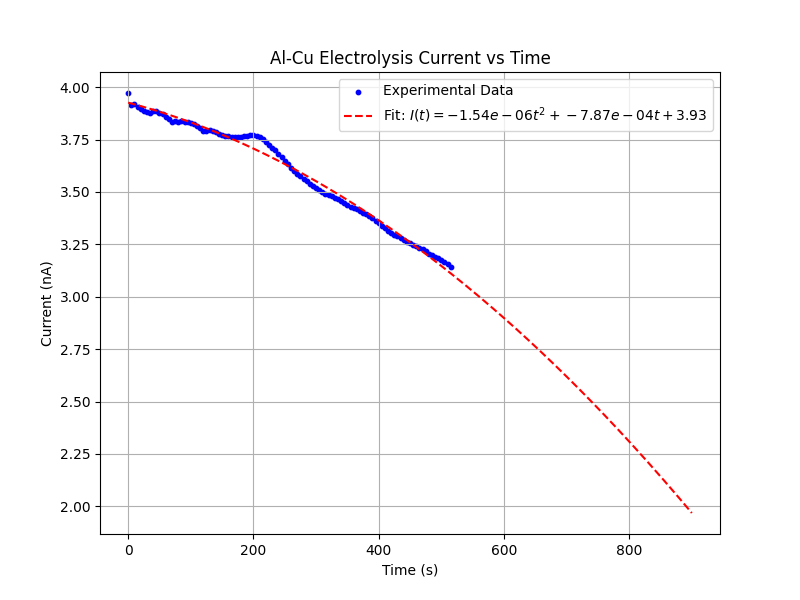
\includegraphics[width=0.78\textwidth]{AlCuRecord/fit_plot.png}
    \caption{Al-Cu 在超纯水中的电流--时间曲线及二次拟合外推}
    \label{fig:alcu-fit}
\end{figure}

Al-Cu 曲线的物理图像是：刚浸入超纯水时，打磨后的 Al 表面仍有较高化学活性，Cu 作为相对惰性的电极提供还原界面，外电路出现微弱电流。随后 Al 表面快速重新生成 $\mathrm{Al_2O_3}$ 钝化膜，膜层提高界面电荷转移电阻；同时超纯水离子浓度极低，局部反应产生的少量离子难以维持较大电导，浓差极化逐渐增强。因此电流缓慢下降但方向不变。曲线中短时起伏可归因于气泡、局部润湿、皮安表量程稳定和环境噪声。

\subsection{Al-Zn 体系}

Al-Zn 初始电流约为 $\SI{1.1875}{\micro A}$，比 Al-Cu 高约三个数量级。前 $\SI{355}{s}$ 内电流从 $\SI{1187.5}{nA}$ 降至 $\SI{36.76}{nA}$，平均衰减速率约为
\begin{equation}
    \bar{v}_{0-355}=\frac{36.76-1187.5}{355}\approx -3.24\ \si{nA.s^{-1}} .
\end{equation}
$t=\SI{360}{s}$ 时仪器显示超量程提示，随后在 $\SI{365}{s}$ 读得 $\SI{22.776}{nA}$，到 $\SI{385}{s}$ 读得 $-\SI{6.622}{nA}$。对过零附近数据线性插值，得到
\begin{equation}
    t_0 \approx \SI{380.1}{s}.
\end{equation}

\begin{figure}[H]
    \centering
    
\includegraphics[width=0.84\textwidth]{AlZnRecord/fit_plot.png}
    \caption{Al-Zn 弱电流测量曲线：上图为全程换算至 $\si{nA}$ 后的变化，下图放大低电流和反向阶段}
    \label{fig:alzn-fit}
\end{figure}

Al-Zn 曲线可分为三个阶段。第一阶段为快速正向衰减：Zn 比 Cu 更活泼，初始时 Zn 与 Al 表面都较新鲜，电极反应强，超纯水中即使只有少量离子也能形成 $\si{\micro A}$ 量级瞬态电流。第二阶段为过零阶段：随着 Zn 溶出、Zn(OH)$_2$ 或氧化产物覆盖表面，Al 表面 $\mathrm{Al_2O_3}$ 膜重新生长，电极附近 pH、溶解氧和金属离子浓度发生空间不均匀分布，界面极化电势逐渐抵消原有电动势。第三阶段为反向稳定阶段：$t=\SI{600}{s}$ 时电流为 $-\SI{196.5}{nA}$，到 $t=\SI{1085}{s}$ 时为 $-\SI{255.3}{nA}$，说明新的界面状态已经主导电流方向，但后期仍受腐蚀产物膜、电解质内阻和扩散限制。

\begin{figure}[H]
    \centering
    \begin{subfigure}{0.31\textwidth}
        \centering
        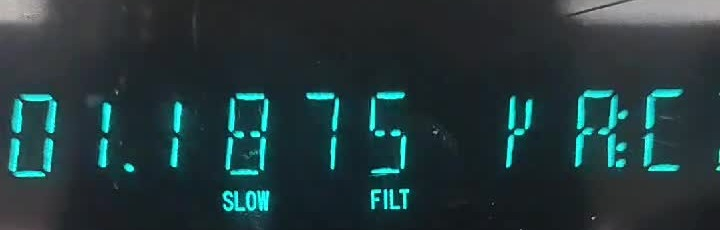
\includegraphics[width=\textwidth]{AlZnRecordFig/figures/display_0001.jpg}
        \caption{$t=\SI{0}{s}$}
    \end{subfigure}
    \hfill
    \begin{subfigure}{0.31\textwidth}
        \centering
        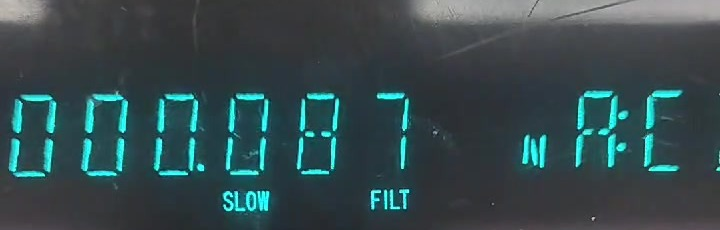
\includegraphics[width=\textwidth]{AlZnRecordFig/figures/display_0077.jpg}
        \caption{$t\approx\SI{380}{s}$}
    \end{subfigure}
    \hfill
    \begin{subfigure}{0.31\textwidth}
        \centering
        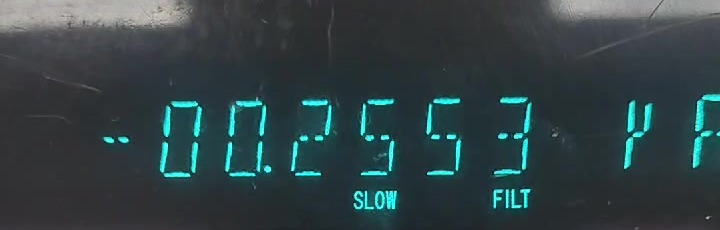
\includegraphics[width=\textwidth]{AlZnRecordFig/figures/display_0218.jpg}
        \caption{$t\approx\SI{1085}{s}$}
    \end{subfigure}
    \caption{Al-Zn 原始显示屏截图示例：初始、过零附近与末段读数}
    \label{fig:alzn-screens}
\end{figure}

对比两组金属电池，Al-Cu 主要体现 Al 钝化导致的弱电流单调衰减；Al-Zn 则体现强初始腐蚀、界面膜重构和浓差极化共同引起的电流反转。超纯水低电导使体系对少量离子和表面膜极其敏感，这是该实验能够观察到细微电化学动力学的关键。

\section{思考题}

\subsection{实验 A 思考题}

\begin{enumerate}
    \item \textbf{为什么 LED 反向连接时能检测光信号？}

    LED 是 PN 结器件。反向偏置时，耗尽层内建电场较强，外电路暗电流很小。当光照进入 PN 结并产生电子--空穴对时，内建电场会把电子和空穴迅速分离，使它们沿相反方向运动，形成反向光生电流。因此 LED 虽然通常用作发光器件，但在反向连接时也可以作为简易光电探测器。光越强，单位时间产生的载流子越多，测得电流越大。

    \item \textbf{如何用此实验设计一个简易光强计？有什么实际应用？}

    可将 LED 固定在遮光盒中，只开一个确定方向的入光孔，反向连接到皮安表或跨阻放大器。先用已知光强标定 $I_{\mathrm{ph}}$ 与光强之间的关系，扣除暗电流后建立校准曲线；之后测未知光源时，根据光生电流反推出相对光强。实际应用包括简易照度计、光通信接收端、遮光报警器、屏幕亮度比较、实验室弱光检测等。若要提高准确度，应固定 LED 角度和距离，并对不同波长分别标定。

    \item \textbf{若实验中发现电流波动大，可能是什么原因？}

    可能原因包括环境光变化、手持光源抖动、光源自身闪烁、LED 接线接触不良、导线和人体引入工频电磁干扰、皮安表未充分预热、量程过小导致接近饱和、空气湿度造成表面漏电以及静电放电。改进方法是使用黑盒遮光、固定光源和 LED、缩短导线、加强屏蔽接地、开启低噪声滤波、等待读数稳定后取平均值。
\end{enumerate}

\subsection{实验 B 思考题}

\begin{enumerate}
    \item \textbf{为什么温度升高会导致漏电流增大？}

    温度升高时，半导体中更多价带电子被热激发到导带，耗尽层中热产生的电子--空穴对数量增加。反向偏置电场会迅速分离这些载流子，形成更大的反向电流。同时高温还会增强表面漏电和缺陷辅助产生电流，因此漏电流常随温度近似指数增长。

    \item \textbf{实验中串联 $\SI{1}{M\Omega}$ 电阻的作用是什么？}

    该电阻主要用于限流保护。当二极管接反、源表设置错误、瞬态冲击或二极管接近击穿时，串联电阻可以限制最大电流，避免损坏皮安表输入端和二极管。它还可以削弱电路中的瞬态充放电电流，使读数更平稳。

    \item \textbf{若漏电流测量结果不稳定（如跳动），可能是什么原因？}

    原因可能包括环境电磁干扰、导线晃动产生摩擦电、屏蔽不充分、接触电阻不稳定、二极管温度尚未稳定、空气湿度导致表面漏电、仪器零点漂移或量程切换引入瞬态。应通过屏蔽盒、短导线、固定夹具、充分预热、恒温等待、ZCOR/ZCHK 校准和多次平均来改善。

    \item \textbf{手机芯片发热时耗电加快，是否与漏电流有关？}

    有关。现代芯片中大量晶体管在关断状态下仍存在亚阈值漏电、栅氧漏电和结漏电。温度升高会增加载流子热激发和亚阈值导通，使静态功耗上升；功耗上升又会继续升温，形成正反馈。因此散热设计不仅影响性能，也直接影响待机功耗和电池续航。
\end{enumerate}

\subsection{实验 C 思考题}

\begin{enumerate}
    \item \textbf{为什么 Al-Zn 电池会出现电流反转，而 Al-Cu 电池不会？请简要描述其背后机理。}

    Al-Zn 的反转来自电极电势差、金属表面膜和局部溶液组成随时间共同演化。初期 Zn 参与的电化学过程较强，形成较大的正向电流；随后 Al 表面快速生成致密 $\mathrm{Al_2O_3}$ 膜，Zn 表面形成氢氧化物或氧化产物，电极附近离子浓度、pH 和溶解氧分布发生变化。这些因素改变两电极的有效界面电势，使原先驱动正向电流的电势差被界面极化抵消并超过，最终出现反向电流。Al-Cu 中 Cu 较稳定，Cu 电极界面不易产生足够强的反向极化，Al 的钝化主要表现为反应速率下降，因此电流只缓慢衰减而不反转。

    \item \textbf{如何通过实验验证 Al 表面氧化膜的绝缘性？}

    可比较新鲜打磨 Al 与自然氧化 Al 的电流响应。先将 Al 打磨后立即与 Cu 或 Zn 组成电池，记录初始电流和衰减曲线；再让同样尺寸的 Al 在空气中静置较长时间，或人为氧化形成更完整膜层，重复相同测量。若氧化膜具有绝缘性，氧化后的 Al 初始电流应显著降低，电流衰减更快或更早进入低电流平台。也可在测量过程中局部刮破 Al 表面氧化膜，若电流瞬时增大并随后再次衰减，则可证明氧化膜对电荷转移具有阻挡作用。

    \item \textbf{若在 Al-Zn 电池的水中加入微量 Cl$^-$（如 $\SI{1}{mM}$ NaCl），初始电流和反向电流会如何变化？为什么？}

    加入 $\mathrm{Cl^-}$ 后，溶液电导率增大，内阻降低，因此初始电流通常会明显增大。同时 $\mathrm{Cl^-}$ 能破坏 Al 表面钝化膜并诱发点蚀，使 Al 的局部溶解和界面电荷转移更容易发生；Zn 的腐蚀也会因离子迁移增强而加快。对反向阶段，$\mathrm{Cl^-}$ 可能加快表面膜破裂和重构，使过零时间提前，反向电流绝对值增大；若腐蚀产物后期大量覆盖电极，也可能使曲线出现新的波动或平台。总体预期是初始电流增大、动力学过程加快，反向电流更容易建立且幅度通常更大。
\end{enumerate}

\end{document}
